\PassOptionsToPackage{unicode=true}{hyperref} % options for packages loaded elsewhere
\PassOptionsToPackage{hyphens}{url}
%
\documentclass[ignorenonframetext,]{beamer}
\usepackage{pgfpages}
\setbeamertemplate{caption}[numbered]
\setbeamertemplate{caption label separator}{: }
\setbeamercolor{caption name}{fg=normal text.fg}
\beamertemplatenavigationsymbolsempty
\usepackage{lmodern}
\usepackage{amssymb,amsmath}
\usepackage{ifxetex,ifluatex}
\usepackage{fixltx2e} % provides \textsubscript
\ifnum 0\ifxetex 1\fi\ifluatex 1\fi=0 % if pdftex
  \usepackage[T1]{fontenc}
  \usepackage[utf8]{inputenc}
  \usepackage{textcomp} % provides euro and other symbols
\else % if luatex or xelatex
  \usepackage{unicode-math}
  \defaultfontfeatures{Ligatures=TeX,Scale=MatchLowercase}
\fi
% use upquote if available, for straight quotes in verbatim environments
\IfFileExists{upquote.sty}{\usepackage{upquote}}{}
% use microtype if available
\IfFileExists{microtype.sty}{%
\usepackage[]{microtype}
\UseMicrotypeSet[protrusion]{basicmath} % disable protrusion for tt fonts
}{}
\IfFileExists{parskip.sty}{%
\usepackage{parskip}
}{% else
\setlength{\parindent}{0pt}
\setlength{\parskip}{6pt plus 2pt minus 1pt}
}
\usepackage{hyperref}
\hypersetup{
            pdftitle={Opportunity in the reproducibility crisis: Computational tools to improve scientific benefaction},
            pdfauthor={Matthew K. Lau, PhD (Harvard Forest)},
            pdfborder={0 0 0},
            breaklinks=true}
\urlstyle{same}  % don't use monospace font for urls
\newif\ifbibliography
\usepackage{longtable,booktabs}
\usepackage{caption}
% These lines are needed to make table captions work with longtable:
\makeatletter
\def\fnum@table{\tablename~\thetable}
\makeatother
\usepackage{graphicx,grffile}
\makeatletter
\def\maxwidth{\ifdim\Gin@nat@width>\linewidth\linewidth\else\Gin@nat@width\fi}
\def\maxheight{\ifdim\Gin@nat@height>\textheight\textheight\else\Gin@nat@height\fi}
\makeatother
% Scale images if necessary, so that they will not overflow the page
% margins by default, and it is still possible to overwrite the defaults
% using explicit options in \includegraphics[width, height, ...]{}
\setkeys{Gin}{width=\maxwidth,height=\maxheight,keepaspectratio}
% Prevent slide breaks in the middle of a paragraph:
\widowpenalties 1 10000
\raggedbottom
\setbeamertemplate{part page}{
\centering
\begin{beamercolorbox}[sep=16pt,center]{part title}
  \usebeamerfont{part title}\insertpart\par
\end{beamercolorbox}
}
\setbeamertemplate{section page}{
\centering
\begin{beamercolorbox}[sep=12pt,center]{part title}
  \usebeamerfont{section title}\insertsection\par
\end{beamercolorbox}
}
\setbeamertemplate{subsection page}{
\centering
\begin{beamercolorbox}[sep=8pt,center]{part title}
  \usebeamerfont{subsection title}\insertsubsection\par
\end{beamercolorbox}
}
\AtBeginPart{
  \frame{\partpage}
}
\AtBeginSection{
  \ifbibliography
  \else
    \frame{\sectionpage}
  \fi
}
\AtBeginSubsection{
  \frame{\subsectionpage}
}
\setlength{\emergencystretch}{3em}  % prevent overfull lines
\providecommand{\tightlist}{%
  \setlength{\itemsep}{0pt}\setlength{\parskip}{0pt}}
\setcounter{secnumdepth}{0}

% set default figure placement to htbp
\makeatletter
\def\fps@figure{htbp}
\makeatother


\title{Opportunity in the reproducibility crisis: Computational tools to
improve scientific benefaction}
\author{Matthew K. Lau, PhD (Harvard Forest)}
\date{}

\begin{document}
\frame{\titlepage}

\begin{frame}

\end{frame}

\begin{frame}{}
\protect\hypertarget{section}{}

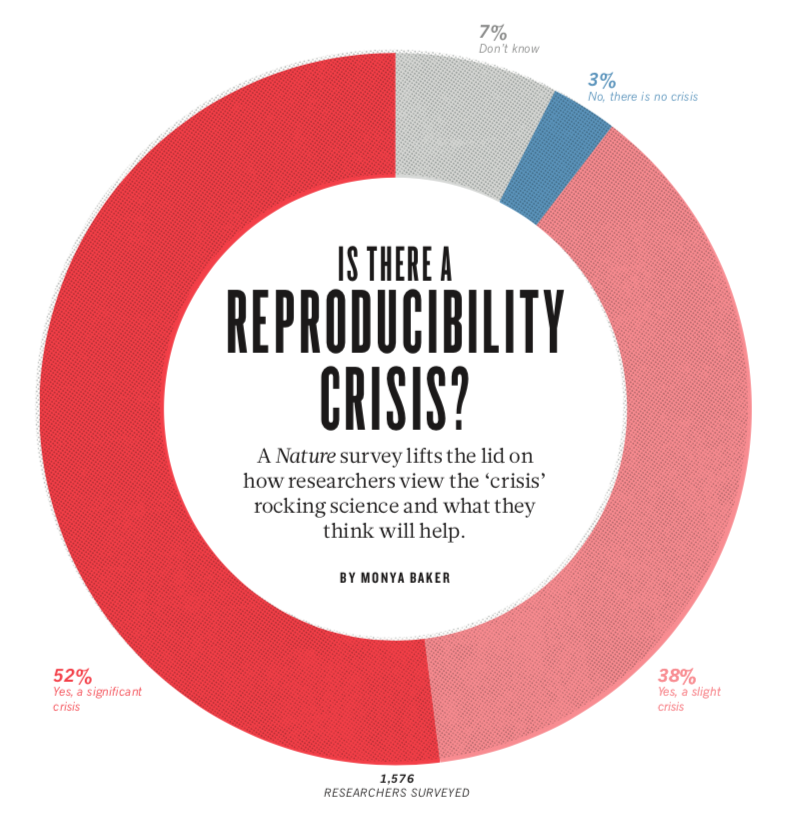
\includegraphics{Baker2016_1.png}

\end{frame}

\begin{frame}{}
\protect\hypertarget{section-1}{}

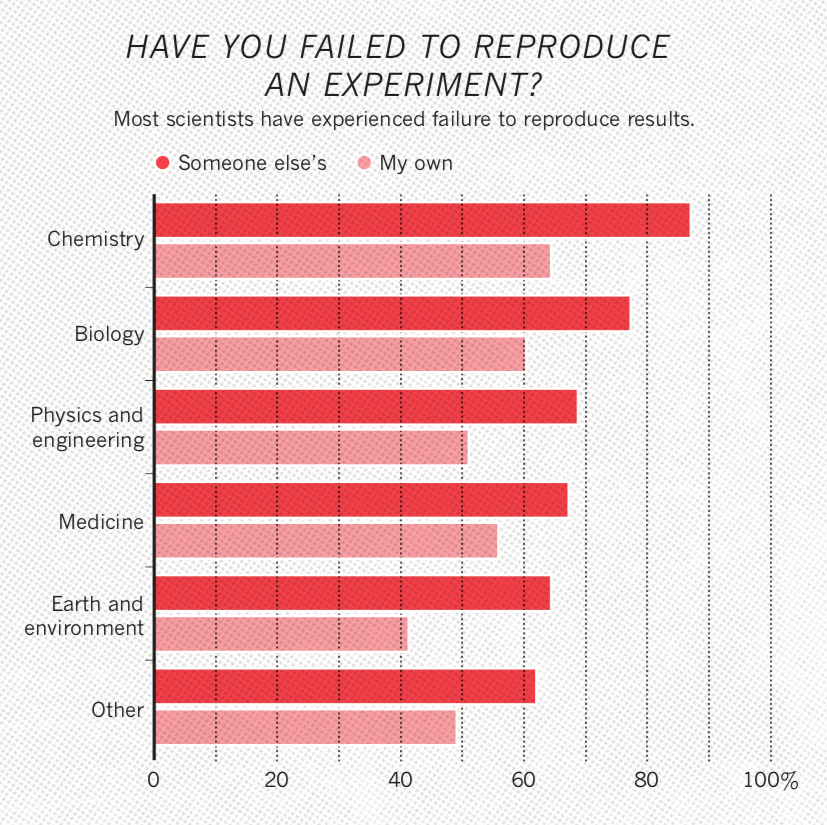
\includegraphics{Baker2016_2.png}

\end{frame}

\begin{frame}{}
\protect\hypertarget{section-2}{}

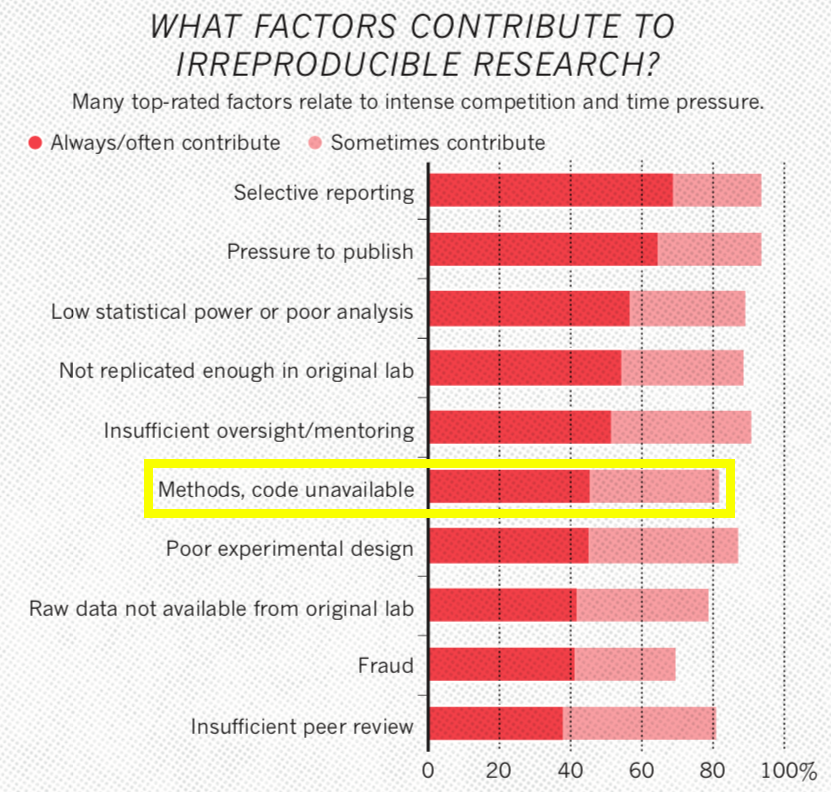
\includegraphics{Baker2016_3.png}

\end{frame}

\begin{frame}{}
\protect\hypertarget{section-3}{}

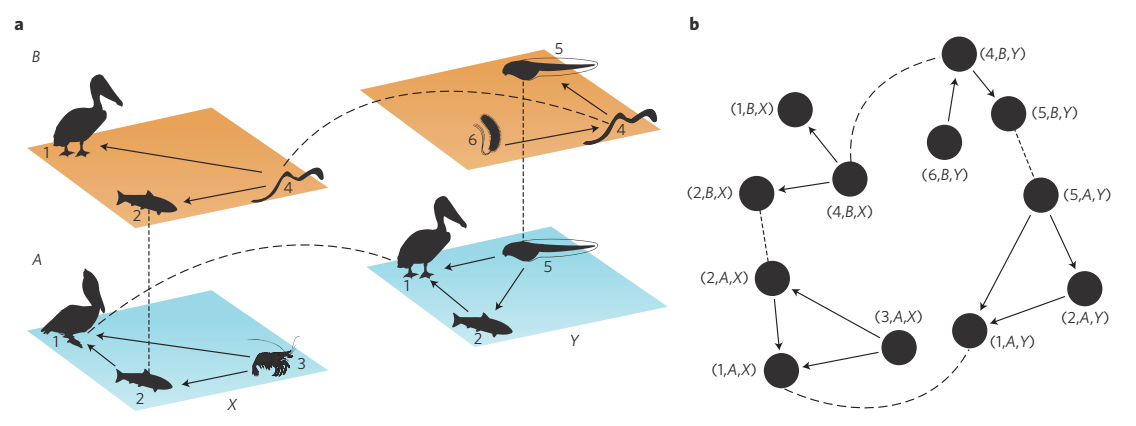
\includegraphics{pilosof1.png}

\end{frame}

\begin{frame}{Motivation: Code in Ecology}
\protect\hypertarget{motivation-code-in-ecology}{}


\includegraphics[width=0.7\textwidth,height=\textheight]{white2016front.png}

\end{frame}

\begin{frame}{Motivation: Ecology Journal Policies}
\protect\hypertarget{motivation-ecology-journal-policies}{}

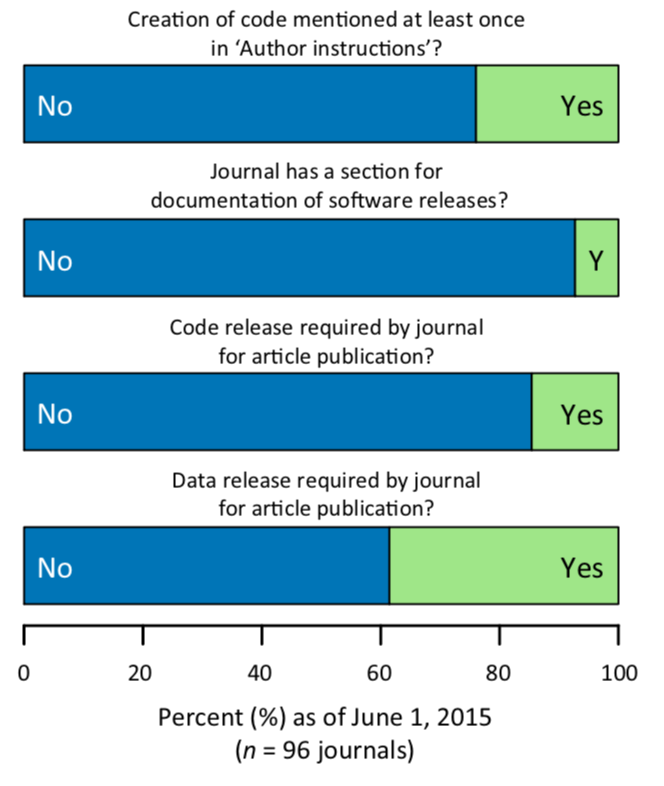
\includegraphics[width=0.5\textwidth,height=\textheight]{white2016.png}

\emph{Meeslan, Heer and White 2016 Trends in Eco Evo}

\end{frame}

\begin{frame}{Motivation: Social Science Journal Policies}
\protect\hypertarget{motivation-social-science-journal-policies}{}

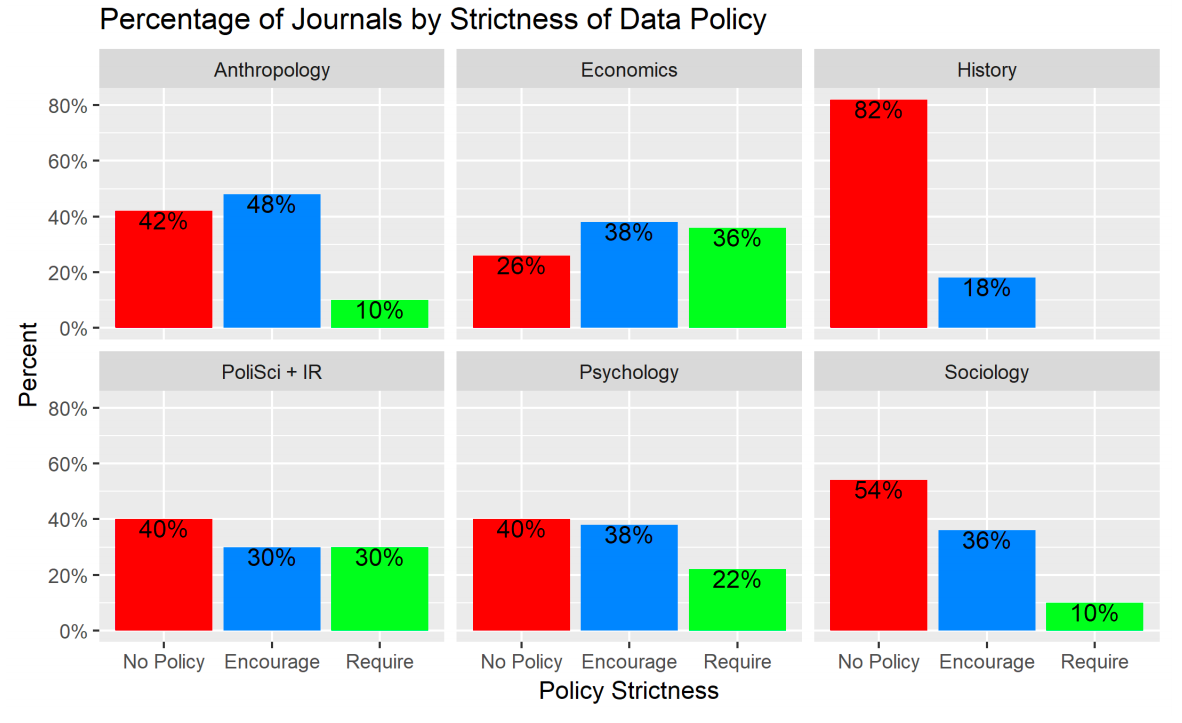
\includegraphics[width=0.7\textwidth,height=\textheight]{crosas2018.png}

\emph{Crosas et al.~2018 SocArXiv}

\end{frame}

\begin{frame}{Motivation: Journal Policy Impacts}
\protect\hypertarget{motivation-journal-policy-impacts}{}


\includegraphics[width=0.7\textwidth,height=\textheight]{Stodden2018front.png}

\end{frame}

\begin{frame}{Motivation: Journal Policy Impacts}
\protect\hypertarget{motivation-journal-policy-impacts-1}{}

\includegraphics[width=0.7\textwidth,height=\textheight]{stodden2018a.png}

\end{frame}

\begin{frame}{Motivation: Journal Policy Impacts}
\protect\hypertarget{motivation-journal-policy-impacts-2}{}

\includegraphics[width=0.7\textwidth,height=\textheight]{stodden2018b.png}

\emph{Stodden et al.~2018 PNAS}

\end{frame}

\begin{frame}{Goal: Repeatability/Reproducibility}
\protect\hypertarget{goal-repeatabilityreproducibility}{}

metadata + data + code + results + contact

\end{frame}

\begin{frame}{Goal: Repeatability/Reproducibility}
\protect\hypertarget{goal-repeatabilityreproducibility-1}{}

BestPractices(metadata + data + code + results + contact)

\end{frame}

\begin{frame}{Goal: Repeatability/Reproducibility}
\protect\hypertarget{goal-repeatabilityreproducibility-2}{}

BestPractices(metadata * data * code * results * contact)

\end{frame}

\begin{frame}{Opportunity: Benefaction not just reproducibility}
\protect\hypertarget{opportunity-benefaction-not-just-reproducibility}{}

\[ Synthesis = f(benefaction) \]

\end{frame}

\begin{frame}{Opportunity: Benefaction not just reproducibility}
\protect\hypertarget{opportunity-benefaction-not-just-reproducibility-1}{}

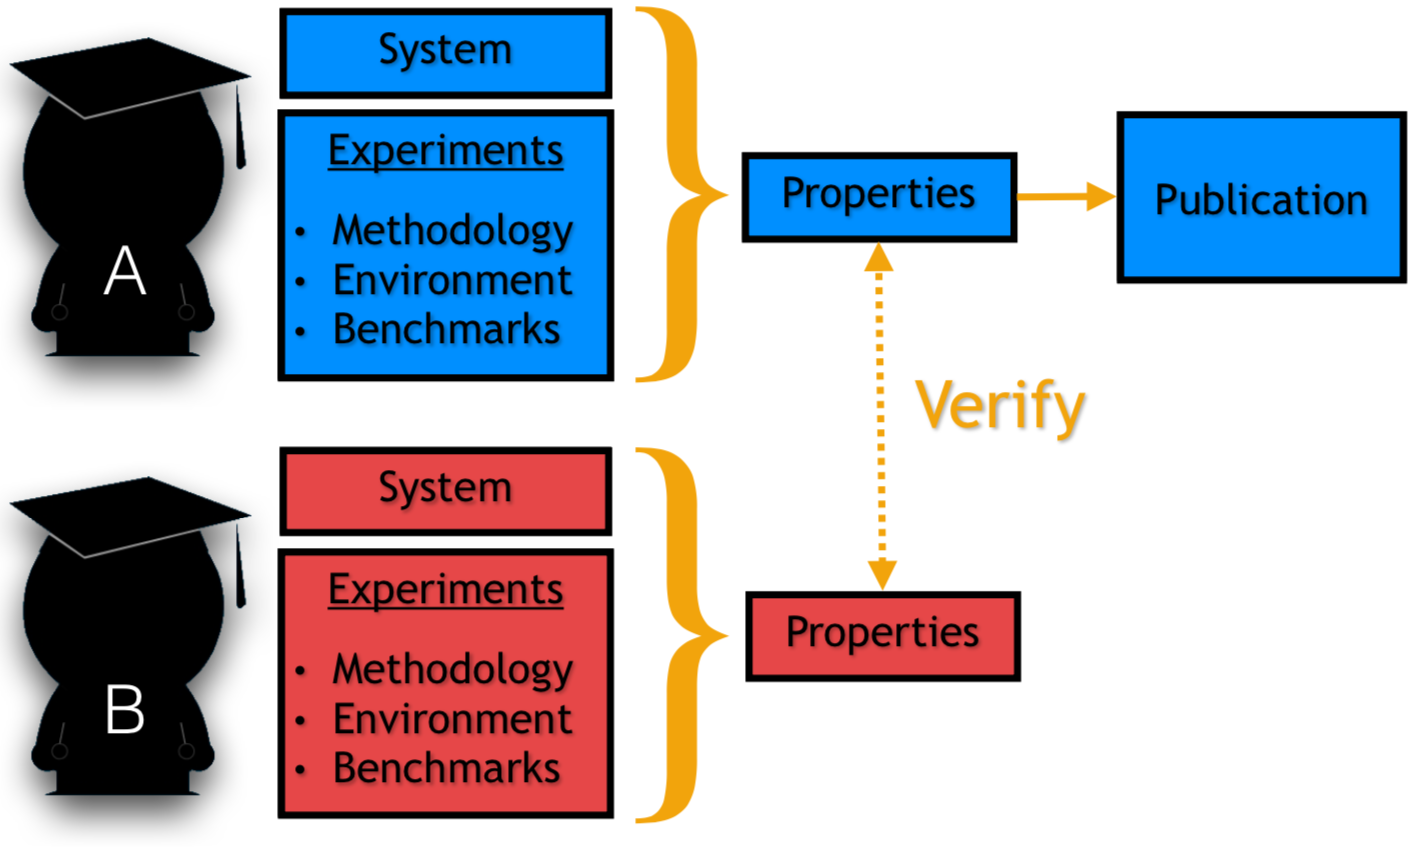
\includegraphics[width=0.7\textwidth,height=\textheight]{colberg_repeat.png}

\emph{Colberg et al.~2015 Comm ACM}

\end{frame}

\begin{frame}{Opportunity: Benefaction not just reproducibility}
\protect\hypertarget{opportunity-benefaction-not-just-reproducibility-2}{}

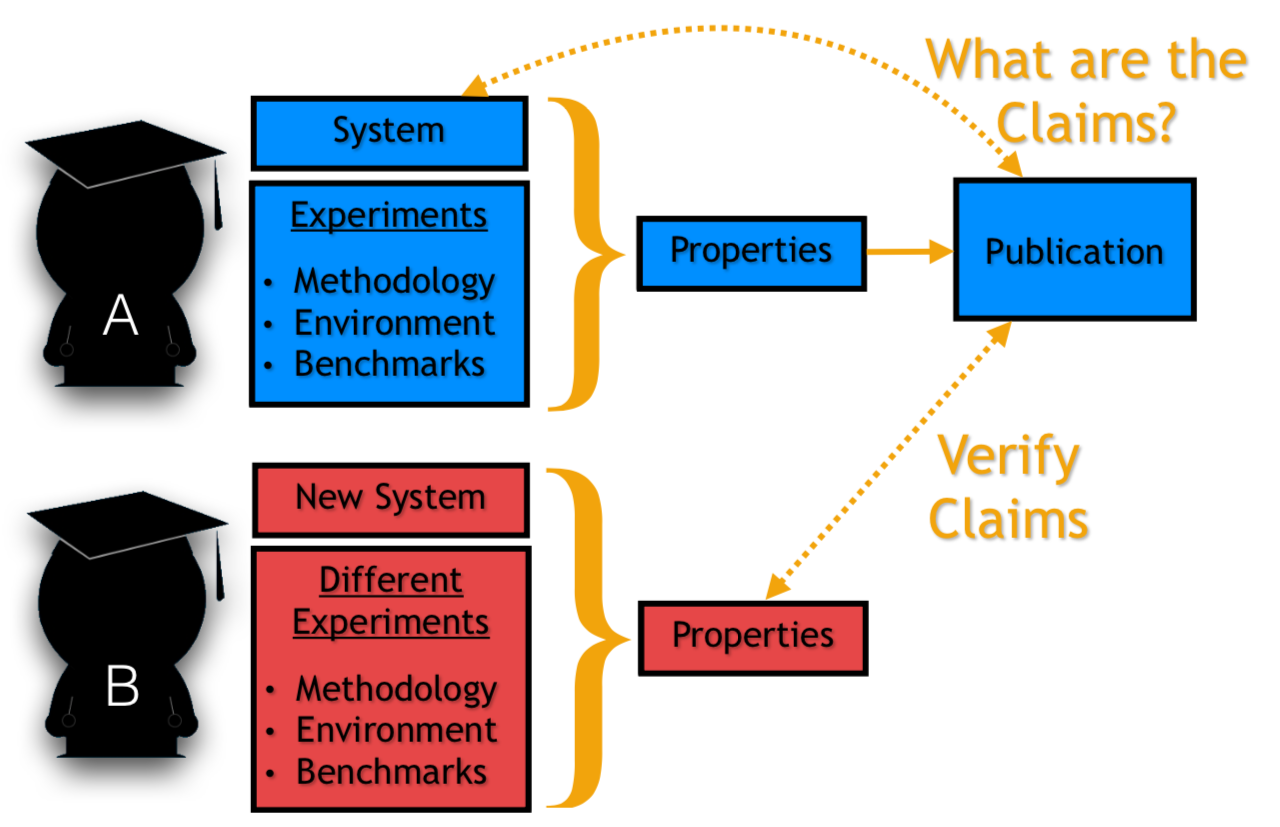
\includegraphics[width=0.7\textwidth,height=\textheight]{colberg_repro.png}

\emph{Colberg et al.~2015 Comm ACM}

\end{frame}

\begin{frame}{Opportunity: Benefaction not just reproducibility}
\protect\hypertarget{opportunity-benefaction-not-just-reproducibility-3}{}

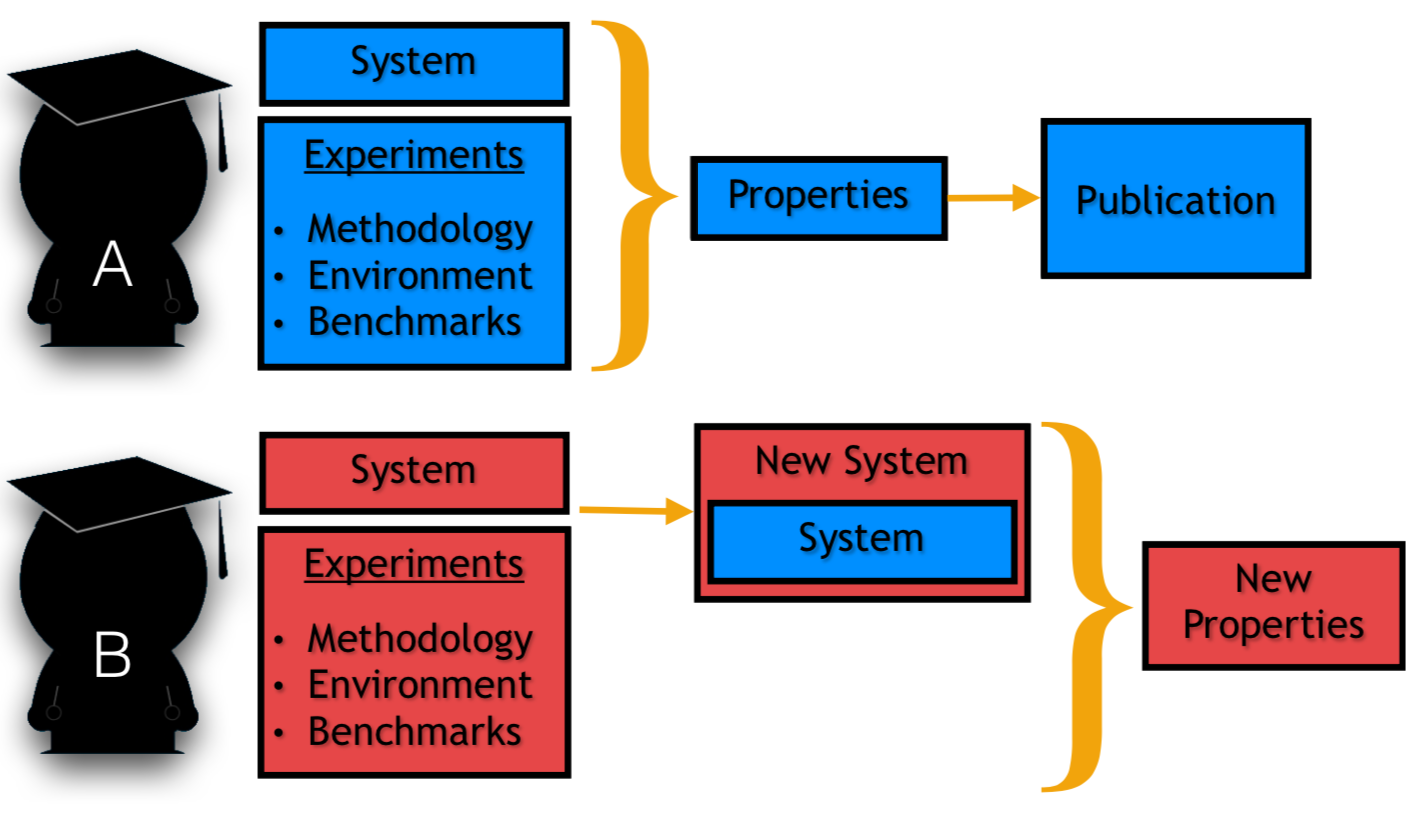
\includegraphics[width=0.7\textwidth,height=\textheight]{colberg_benefact.png}

\emph{Colberg et al.~2015 Comm ACM}

\end{frame}

\begin{frame}{Tools: Research Pipeline}
\protect\hypertarget{tools-research-pipeline}{}

\begin{longtable}[]{@{}lllll@{}}
\toprule
\begin{minipage}[b]{0.07\columnwidth}\raggedright
Thought\strut
\end{minipage} & \begin{minipage}[b]{0.18\columnwidth}\raggedright
Data Collection\strut
\end{minipage} & \begin{minipage}[b]{0.20\columnwidth}\raggedright
Data Processing\strut
\end{minipage} & \begin{minipage}[b]{0.23\columnwidth}\raggedright
Analysis\strut
\end{minipage} & \begin{minipage}[b]{0.18\columnwidth}\raggedright
Reporting\strut
\end{minipage}\tabularnewline
\midrule
\endhead
\begin{minipage}[t]{0.07\columnwidth}\raggedright
\emph{Meta-Data}\strut
\end{minipage} & \begin{minipage}[t]{0.18\columnwidth}\raggedright
\emph{Meta-Data} + \emph{Provenance}\strut
\end{minipage} & \begin{minipage}[t]{0.20\columnwidth}\raggedright
\emph{Provenance} + \emph{Versioning}\strut
\end{minipage} & \begin{minipage}[t]{0.23\columnwidth}\raggedright
\emph{Versioning} + \emph{Provenance}\strut
\end{minipage} & \begin{minipage}[t]{0.18\columnwidth}\raggedright
\emph{Lit Prog} + \emph{Versioning}\strut
\end{minipage}\tabularnewline
\bottomrule
\end{longtable}

\end{frame}

\begin{frame}{Tools: Overview}
\protect\hypertarget{tools-overview}{}

\begin{longtable}[]{@{}lcccccccc@{}}
\toprule
\begin{minipage}[b]{0.12\columnwidth}\raggedright
\strut
\end{minipage} & \begin{minipage}[b]{0.05\columnwidth}\centering
Dataverse\strut
\end{minipage} & \begin{minipage}[b]{0.05\columnwidth}\centering
Code Ocean\strut
\end{minipage} & \begin{minipage}[b]{0.05\columnwidth}\centering
Zenodo\strut
\end{minipage} & \begin{minipage}[b]{0.07\columnwidth}\centering
Figshare\strut
\end{minipage} & \begin{minipage}[b]{0.04\columnwidth}\centering
Dryad\strut
\end{minipage} & \begin{minipage}[b]{0.06\columnwidth}\centering
PANGAEA\strut
\end{minipage} & \begin{minipage}[b]{0.15\columnwidth}\centering
GitHub \& Bitbucket\strut
\end{minipage} & \begin{minipage}[b]{0.18\columnwidth}\centering
Supplementary Material\strut
\end{minipage}\tabularnewline
\midrule
\endhead
\begin{minipage}[t]{0.12\columnwidth}\raggedright
Meta Data\strut
\end{minipage} & \begin{minipage}[t]{0.05\columnwidth}\centering
Yes\strut
\end{minipage} & \begin{minipage}[t]{0.05\columnwidth}\centering
Yes\strut
\end{minipage} & \begin{minipage}[t]{0.05\columnwidth}\centering
Yes\strut
\end{minipage} & \begin{minipage}[t]{0.07\columnwidth}\centering
Yes\strut
\end{minipage} & \begin{minipage}[t]{0.04\columnwidth}\centering
Yes\strut
\end{minipage} & \begin{minipage}[t]{0.06\columnwidth}\centering
Yes\strut
\end{minipage} & \begin{minipage}[t]{0.15\columnwidth}\centering
Yes\strut
\end{minipage} & \begin{minipage}[t]{0.18\columnwidth}\centering
Yes\strut
\end{minipage}\tabularnewline
\begin{minipage}[t]{0.12\columnwidth}\raggedright
Data Hosting\strut
\end{minipage} & \begin{minipage}[t]{0.05\columnwidth}\centering
Yes\strut
\end{minipage} & \begin{minipage}[t]{0.05\columnwidth}\centering
Yes\strut
\end{minipage} & \begin{minipage}[t]{0.05\columnwidth}\centering
Yes\strut
\end{minipage} & \begin{minipage}[t]{0.07\columnwidth}\centering
Yes\strut
\end{minipage} & \begin{minipage}[t]{0.04\columnwidth}\centering
Yes\strut
\end{minipage} & \begin{minipage}[t]{0.06\columnwidth}\centering
Yes\strut
\end{minipage} & \begin{minipage}[t]{0.15\columnwidth}\centering
Yes\strut
\end{minipage} & \begin{minipage}[t]{0.18\columnwidth}\centering
Yes\strut
\end{minipage}\tabularnewline
\begin{minipage}[t]{0.12\columnwidth}\raggedright
Code Hosting\strut
\end{minipage} & \begin{minipage}[t]{0.05\columnwidth}\centering
Yes\strut
\end{minipage} & \begin{minipage}[t]{0.05\columnwidth}\centering
Yes\strut
\end{minipage} & \begin{minipage}[t]{0.05\columnwidth}\centering
Yes\strut
\end{minipage} & \begin{minipage}[t]{0.07\columnwidth}\centering
No\strut
\end{minipage} & \begin{minipage}[t]{0.04\columnwidth}\centering
No\strut
\end{minipage} & \begin{minipage}[t]{0.06\columnwidth}\centering
No\strut
\end{minipage} & \begin{minipage}[t]{0.15\columnwidth}\centering
Yes\strut
\end{minipage} & \begin{minipage}[t]{0.18\columnwidth}\centering
Yes\strut
\end{minipage}\tabularnewline
\begin{minipage}[t]{0.12\columnwidth}\raggedright
Versioning\strut
\end{minipage} & \begin{minipage}[t]{0.05\columnwidth}\centering
No?\strut
\end{minipage} & \begin{minipage}[t]{0.05\columnwidth}\centering
No?\strut
\end{minipage} & \begin{minipage}[t]{0.05\columnwidth}\centering
Yes\strut
\end{minipage} & \begin{minipage}[t]{0.07\columnwidth}\centering
No\strut
\end{minipage} & \begin{minipage}[t]{0.04\columnwidth}\centering
No\strut
\end{minipage} & \begin{minipage}[t]{0.06\columnwidth}\centering
No\strut
\end{minipage} & \begin{minipage}[t]{0.15\columnwidth}\centering
Yes\strut
\end{minipage} & \begin{minipage}[t]{0.18\columnwidth}\centering
No\strut
\end{minipage}\tabularnewline
\begin{minipage}[t]{0.12\columnwidth}\raggedright
Capsules\strut
\end{minipage} & \begin{minipage}[t]{0.05\columnwidth}\centering
No\strut
\end{minipage} & \begin{minipage}[t]{0.05\columnwidth}\centering
Yes\strut
\end{minipage} & \begin{minipage}[t]{0.05\columnwidth}\centering
No\strut
\end{minipage} & \begin{minipage}[t]{0.07\columnwidth}\centering
No\strut
\end{minipage} & \begin{minipage}[t]{0.04\columnwidth}\centering
No\strut
\end{minipage} & \begin{minipage}[t]{0.06\columnwidth}\centering
No\strut
\end{minipage} & \begin{minipage}[t]{0.15\columnwidth}\centering
No\strut
\end{minipage} & \begin{minipage}[t]{0.18\columnwidth}\centering
No\strut
\end{minipage}\tabularnewline
\begin{minipage}[t]{0.12\columnwidth}\raggedright
Assigns DOI\strut
\end{minipage} & \begin{minipage}[t]{0.05\columnwidth}\centering
Yes\strut
\end{minipage} & \begin{minipage}[t]{0.05\columnwidth}\centering
Yes\strut
\end{minipage} & \begin{minipage}[t]{0.05\columnwidth}\centering
Yes\strut
\end{minipage} & \begin{minipage}[t]{0.07\columnwidth}\centering
Yes\strut
\end{minipage} & \begin{minipage}[t]{0.04\columnwidth}\centering
Yes\strut
\end{minipage} & \begin{minipage}[t]{0.06\columnwidth}\centering
Yes\strut
\end{minipage} & \begin{minipage}[t]{0.15\columnwidth}\centering
No\strut
\end{minipage} & \begin{minipage}[t]{0.18\columnwidth}\centering
No\strut
\end{minipage}\tabularnewline
\begin{minipage}[t]{0.12\columnwidth}\raggedright
License\strut
\end{minipage} & \begin{minipage}[t]{0.05\columnwidth}\centering
Flexible\strut
\end{minipage} & \begin{minipage}[t]{0.05\columnwidth}\centering
Flexible\strut
\end{minipage} & \begin{minipage}[t]{0.05\columnwidth}\centering
Flexible\strut
\end{minipage} & \begin{minipage}[t]{0.07\columnwidth}\centering
MIT\strut
\end{minipage} & \begin{minipage}[t]{0.04\columnwidth}\centering
CC0\strut
\end{minipage} & \begin{minipage}[t]{0.06\columnwidth}\centering
CC-BY\strut
\end{minipage} & \begin{minipage}[t]{0.15\columnwidth}\centering
Flexible\strut
\end{minipage} & \begin{minipage}[t]{0.18\columnwidth}\centering
None\strut
\end{minipage}\tabularnewline
\begin{minipage}[t]{0.12\columnwidth}\raggedright
Cost\strut
\end{minipage} & \begin{minipage}[t]{0.05\columnwidth}\centering
None\strut
\end{minipage} & \begin{minipage}[t]{0.05\columnwidth}\centering
Possible\strut
\end{minipage} & \begin{minipage}[t]{0.05\columnwidth}\centering
None\strut
\end{minipage} & \begin{minipage}[t]{0.07\columnwidth}\centering
None\strut
\end{minipage} & \begin{minipage}[t]{0.04\columnwidth}\centering
Possible\strut
\end{minipage} & \begin{minipage}[t]{0.06\columnwidth}\centering
None\strut
\end{minipage} & \begin{minipage}[t]{0.15\columnwidth}\centering
None\strut
\end{minipage} & \begin{minipage}[t]{0.18\columnwidth}\centering
None\strut
\end{minipage}\tabularnewline
\bottomrule
\end{longtable}

\emph{Adapted from Mislan, Heer \& White 2016 Trends in Ecol Evol}

\end{frame}

\begin{frame}{Reality: Common Ground}
\protect\hypertarget{reality-common-ground}{}

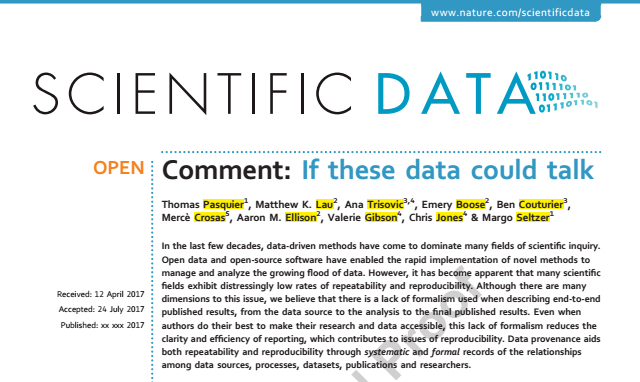
\includegraphics[width=0.7\textwidth,height=\textheight]{nsd.png}

\end{frame}

\begin{frame}{Reality: Common Ground}
\protect\hypertarget{reality-common-ground-1}{}

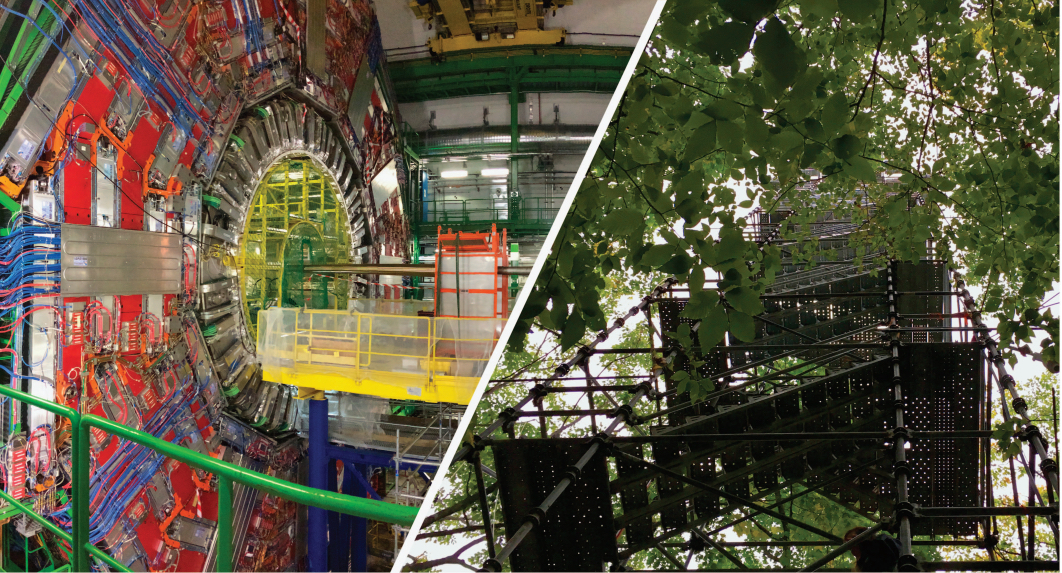
\includegraphics[width=0.7\textwidth,height=\textheight]{cern_hf.png}

\end{frame}

\begin{frame}{Reality: Common Ground}
\protect\hypertarget{reality-common-ground-2}{}

\begin{itemize}
\tightlist
\item
  \emph{Most scientists don't want to produce software, they want to do
  science.}
\end{itemize}

\end{frame}

\begin{frame}{Reality: Common Ground}
\protect\hypertarget{reality-common-ground-3}{}

\begin{itemize}
\item
  \emph{Most scientists don't want to produce software, they want to do
  science.}
\item
  \emph{Let's automate as much of the process as we can to lower
  activation energy, decrease error rates and increase sharing.}
\end{itemize}

\end{frame}

\begin{frame}{Tools: Encapsulator}
\protect\hypertarget{tools-encapsulator}{}

\begin{figure}
\centering
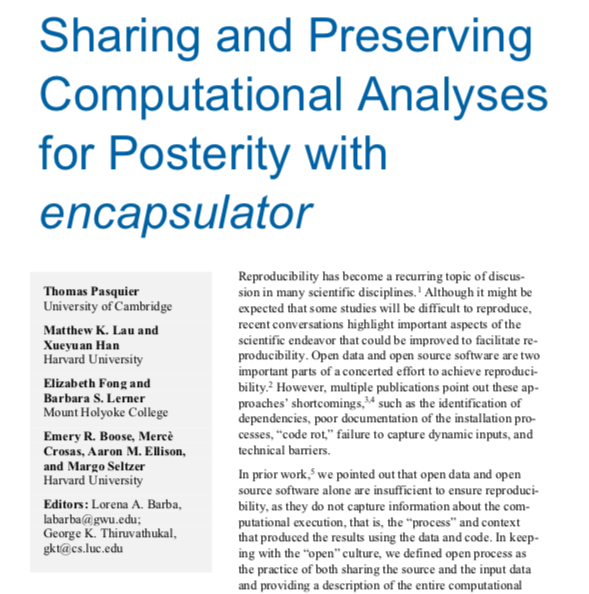
\includegraphics{CISE2018.png}
\caption{IEEE: Computing in Science \& Engineering 2018}
\end{figure}

\end{frame}

\begin{frame}{Tools: Encapsulator}
\protect\hypertarget{tools-encapsulator-1}{}

Goal: Simplify computational reproducibility

\begin{enumerate}
\tightlist
\item
  Create a data ``capsule'' with code, data and environment
\end{enumerate}

\end{frame}

\begin{frame}{Tools: Encapsulator}
\protect\hypertarget{tools-encapsulator-2}{}

Goal: Simplify computational reproducibility

\begin{enumerate}
\tightlist
\item
  Create a data ``capsule'' with code, data and environment
\item
  Increase transparency with ``cleaned'' code and workspace
\end{enumerate}

\end{frame}

\begin{frame}{}
\protect\hypertarget{section-4}{}

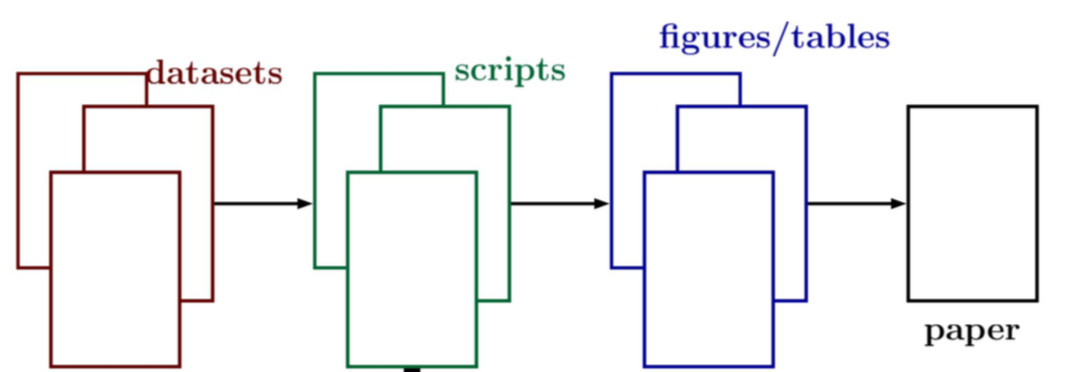
\includegraphics[width=0.7\textwidth,height=\textheight]{cise1.png}

\end{frame}

\begin{frame}{}
\protect\hypertarget{section-5}{}

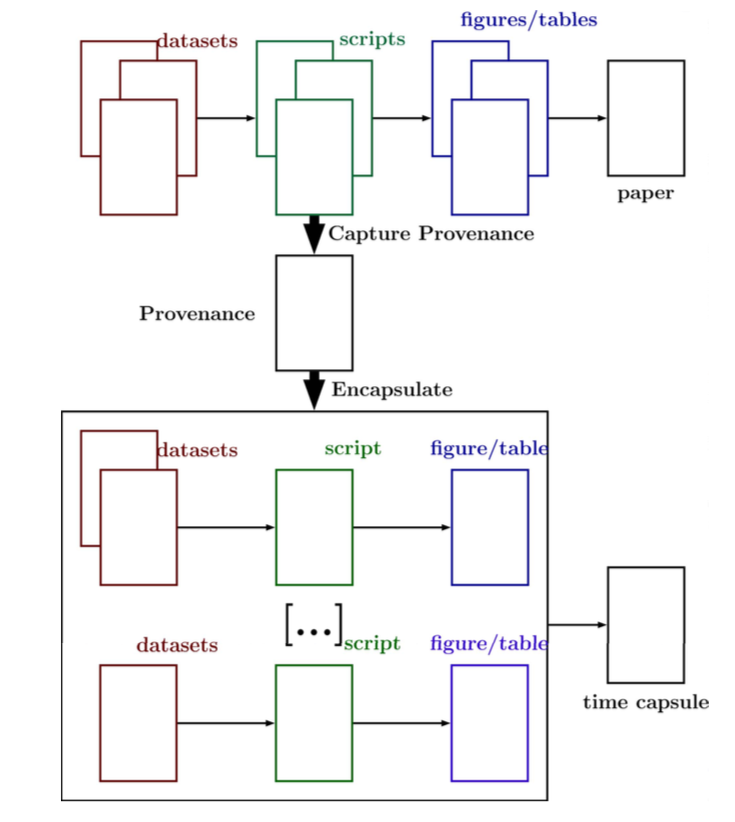
\includegraphics[width=0.5\textwidth,height=\textheight]{cise2.png}

\end{frame}

\begin{frame}{What is data provenance?}
\protect\hypertarget{what-is-data-provenance}{}

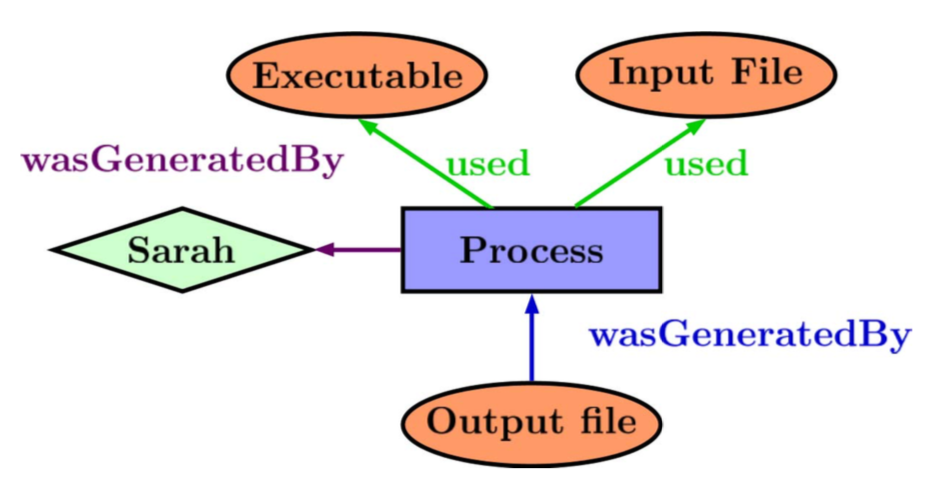
\includegraphics[width=0.8\textwidth,height=\textheight]{provw3c.png}

\end{frame}

\begin{frame}{What is data provenance?}
\protect\hypertarget{what-is-data-provenance-1}{}

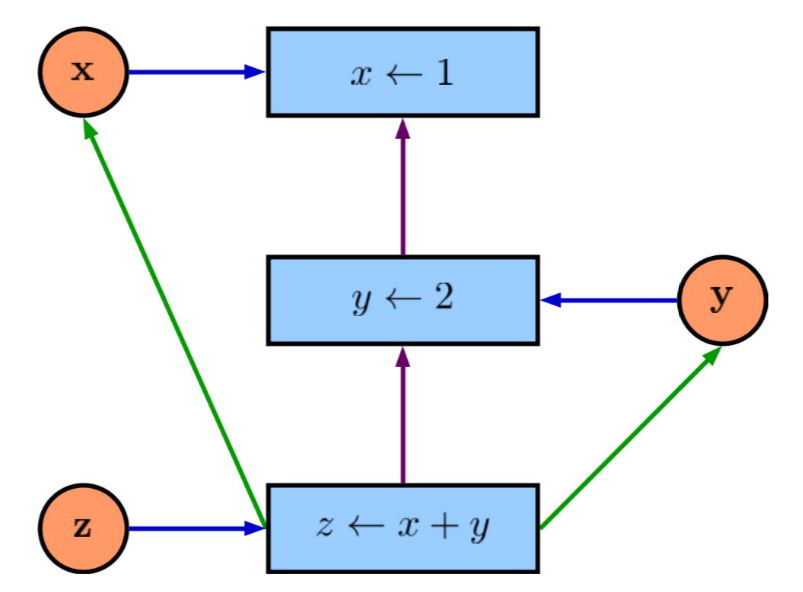
\includegraphics[width=0.5\textwidth,height=\textheight]{provEx.png}

\end{frame}

\begin{frame}{Prov. Huh. What is it good for?}
\protect\hypertarget{prov.-huh.-what-is-it-good-for}{}

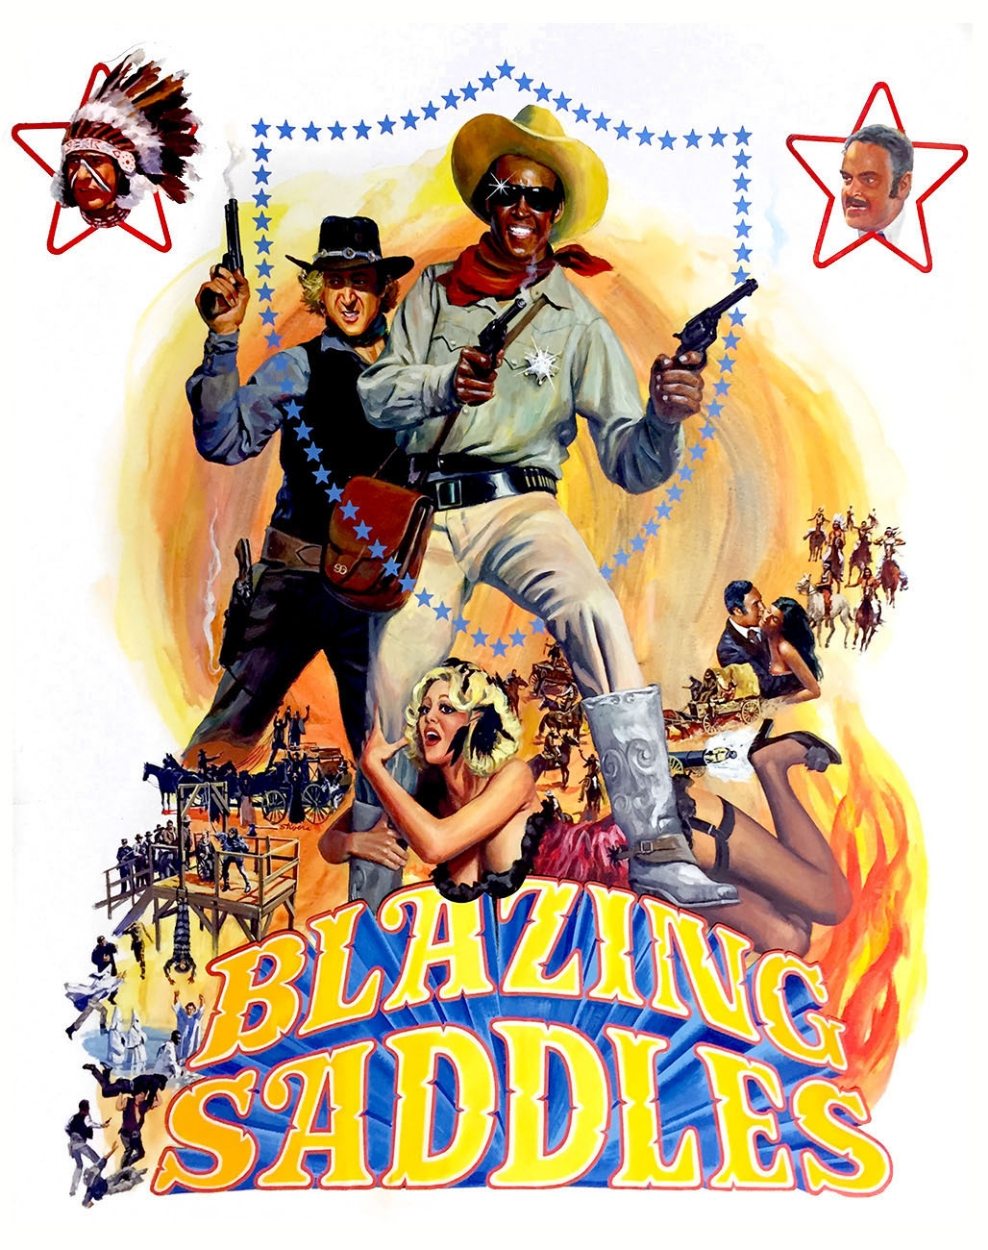
\includegraphics{blazing_saddles2.JPG}

\end{frame}

\begin{frame}{Prov. Huh. What is it good for?}
\protect\hypertarget{prov.-huh.-what-is-it-good-for-1}{}

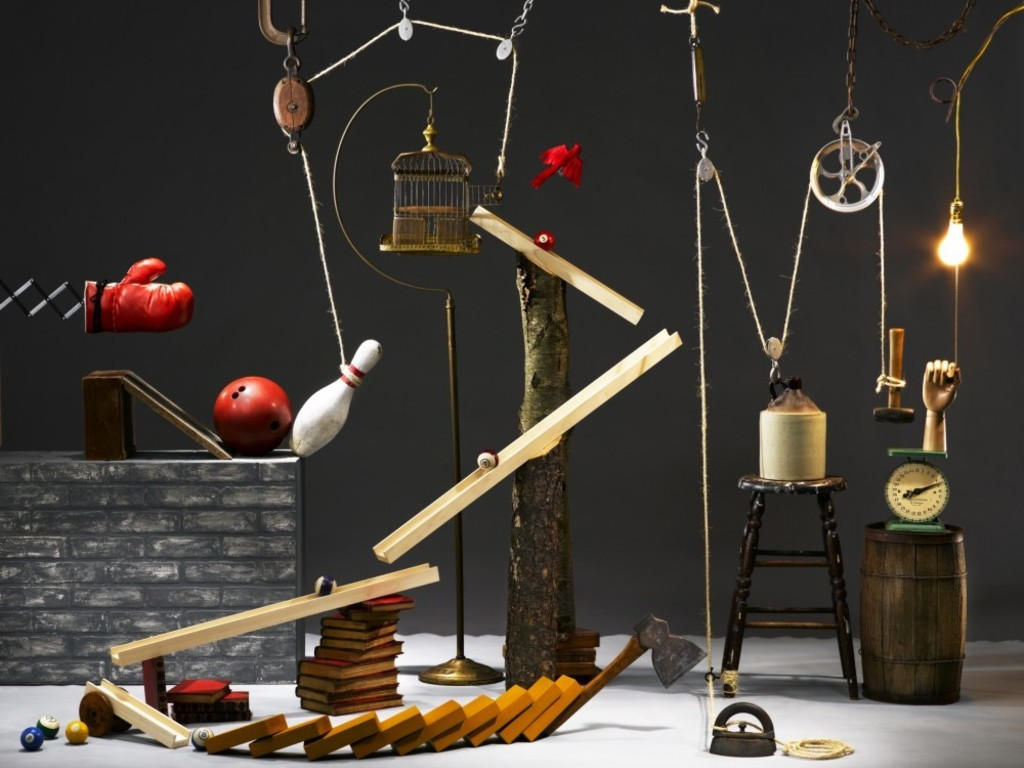
\includegraphics{rgm.jpg}

\end{frame}

\begin{frame}{Prov. Huh. What is it good for?}
\protect\hypertarget{prov.-huh.-what-is-it-good-for-2}{}

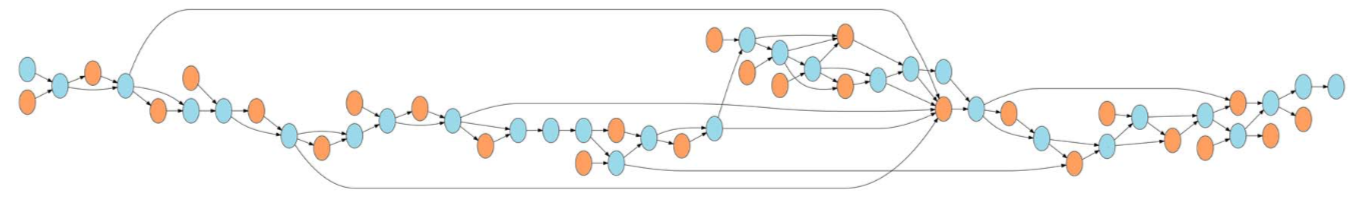
\includegraphics[width=1\textwidth,height=\textheight]{messy1.png}

\end{frame}

\begin{frame}{Prov. Huh. What is it good for?}
\protect\hypertarget{prov.-huh.-what-is-it-good-for-3}{}

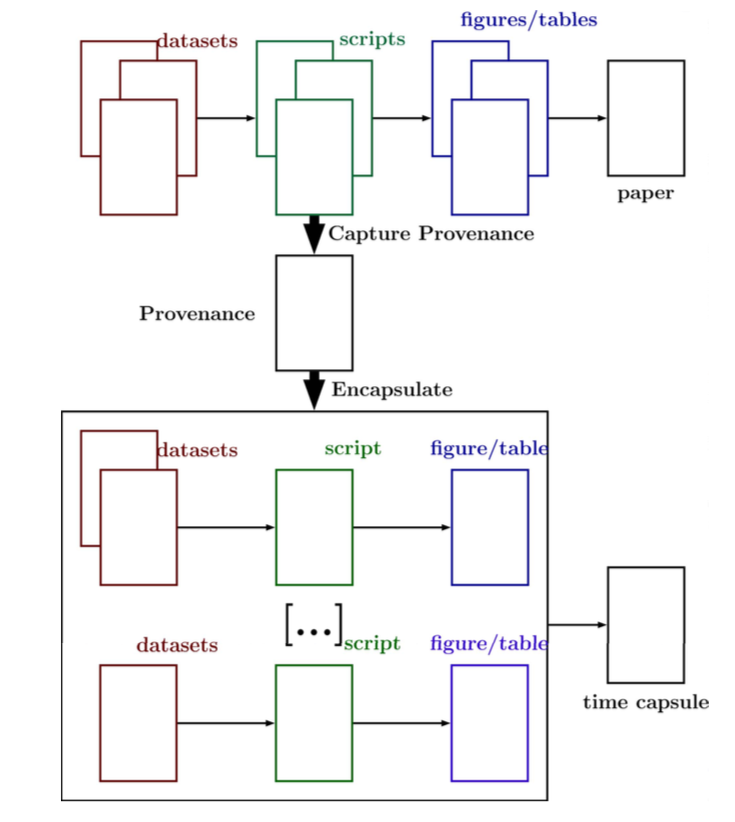
\includegraphics[width=0.4\textwidth,height=\textheight]{cise2.png}

\end{frame}

\begin{frame}{encapsulator(A Kit of Parts): Checking inputs and outputs}
\protect\hypertarget{encapsulatora-kit-of-parts-checking-inputs-and-outputs}{}

\begin{itemize}
\tightlist
\item
  \emph{lintR} (Hester 2017)
\item
  \emph{containR} (Chen 2018)
\end{itemize}

\end{frame}

\begin{frame}{encapsulator(A Kit of Parts): Code Formatting}
\protect\hypertarget{encapsulatora-kit-of-parts-code-formatting}{}

\begin{itemize}
\tightlist
\item
  \emph{formatR} (Xie 2017)
\item
  \emph{styler} (Muller \& Walther 2018)
\end{itemize}

\end{frame}

\begin{frame}{encapsulator(A Kit of Parts): Code Cleaning}
\protect\hypertarget{encapsulatora-kit-of-parts-code-cleaning}{}

\begin{itemize}
\tightlist
\item
  \emph{Rclean} (Lau 2018)
\item
  \emph{CodeDepends} (Lang et al.~2018)
\end{itemize}

\end{frame}

\begin{frame}{encapsulator(A Kit of Parts): Capsule creation}
\protect\hypertarget{encapsulatora-kit-of-parts-capsule-creation}{}

\begin{itemize}
\tightlist
\item
  Virtual Machine (encapsulator)
\item
  Docker (containR)
\item
  Literate computing notebook (Jupyter)
\item
  Compressed (Reprozip)
\item
  Capsule database (Code Ocean)
\end{itemize}

\end{frame}

\begin{frame}{Conclusion: The next great challenge is synthesis}
\protect\hypertarget{conclusion-the-next-great-challenge-is-synthesis}{}

** Software should not limit science **

\end{frame}

\begin{frame}{Conclusion: The next great challenge is synthesis}
\protect\hypertarget{conclusion-the-next-great-challenge-is-synthesis-1}{}

\includegraphics[width=0.2\textwidth,height=\textheight]{dataverse_world.png}

\end{frame}

\begin{frame}{Questions and Discussion:}
\protect\hypertarget{questions-and-discussion}{}

\emph{Possible discussion topics:}


\includegraphics[width=0.2\textwidth,height=\textheight]{dataverse_r_project.png}

\begin{enumerate}
\tightlist
\item
  What checks are in place to verify and link dataverses?
\item
  Can provenance production become a part of the checking system?
\item
  What are the pros and cons of automated checking/verification and/or
  cleaning/encapsulation of dataverses?
\item
  I'm focused on R's wild-wild-west, but how does this translate to
  other languages?
\end{enumerate}

\emph{Contact Info:}

\textbf{Email:
\emph{\href{mailto:matthewklau@fas.harvard.edu}{\nolinkurl{matthewklau@fas.harvard.edu}}}}

\textbf{Github: MKLau}

\textbf{Slack: MKLau}

\emph{Much of this work was supported by NSF SSI-1450277 (End-to-End
Provenance) and ACI-1448123 (Citation++).} \emph{More details are
available at
\url{https://projects.iq.harvard.edu/provenance-at-harvard}}


\includegraphics[width=0.19\textwidth,height=\textheight]{inst_2.png}

\includegraphics[width=0.2\textwidth,height=\textheight]{inst_3.png}

\includegraphics[width=0.25\textwidth,height=\textheight]{inst_1.png}

\includegraphics[width=0.15\textwidth,height=\textheight]{inst_4.png}

\end{frame}

\end{document}
